\chapter{预备知识}
本文中考虑的是 $\mathbb R^d$ 中的有界开集 $\Omega$
上的问题。
虚单元方法与有限元方法类似,需要将 $\Omega$ 剖分为多面体网格。
在本章节中我们给出一些本文中使用的预备知识,包括符号约定、基本的网格假设、
一些常用的不等式和本文涉及的虚单元空间等。

\section{符号约定}
在本文中,$\mathbb{N}$ 表示所有非负整数的集合。
$\#S$ 表示集合 $S$ 中元素的个数。 $\mathbb{R}^d$ 表示 $d$ 维欧式空间。
$\mathrm{dim}(V)$ 表示向量空间 $V$ 的维数。

多重指标是一个非常基础的概念,不仅可以用来简化公式表达,
而且与多项式一一对应,在理论分析和数值计算都有应用。
一个长度为 $n$ 的多重指标是一个非负整数数组:
$$
\boldsymbol\alpha = (\alpha_0, \alpha_1, \ldots, \alpha_{n-1}), \quad \alpha_i
\in \mathbb{N}, i=0, \ldots, n-1.
$$
定义多重指标的阶为其元素之和:
$
|\boldsymbol \alpha| = \sum_{i = 0}^{n-1} \alpha_i,
$
其阶乘定义为
$
\boldsymbol \alpha! = \prod_{i=0}^n (\alpha_i!).
$
所有长度为 $n$ 且阶数为 $k$ 的多重指标集合记作 $\mathbb{T}^n_k$,即
$$
\mathbb{T}^n_k = \{ \boldsymbol \alpha \in \mathbb{N}^{n+1}: |\boldsymbol \alpha| = k\}.
$$
所有阶数小于等于 $k$ 的多重指标集合记作 $\mathbb{T}^n_{\leq k}$,即:
$$
\mathbb{T}^n_{\leq k} = \{ \boldsymbol \alpha \in \mathbb{N}^{n+1}: |\boldsymbol
\alpha| \leq k\}.
$$
%在本文中 $\mathbb{T}^n_k$ 中的元素通过字典顺序进行排列:
%\begin{equation*}
%R_n(\boldsymbol \alpha) = \sum_{i=1}^n{\alpha_i + \alpha_{i+1} + \cdots + \alpha_n + n - i \choose n + 1 - i}.
%\end{equation*}
%比如对于 $\mathbb{T}^3_4$,前四个多重指标为:
%$$\begin{matrix}
%0 : \\
%1 : \\
%2 : \\
%3 : \\
%\end{matrix}
%\begin{pmatrix}
%    4 & 0 & 0  \\
%    3 & 1 & 0  \\
%    3 & 0 & 1  \\
%    2 & 2 & 0  \\
%\end{pmatrix}.$$
%注意,$\alpha_0$ 在计算 $R_n(\boldsymbol \alpha)$ 时并未使用。

下面给出本文中使用的张量空间相关的定义和引理。
定义 $d$ 维空间中的 $r$ 阶张量空间为 $(\mathbb{R}^d)^{ r}$,对于 
$\boldsymbol{\tau} \in (\mathbb{R}^d)^{ r}$,可以写为分量形式:
$$
\btau = \tau_{i_0, i_1, \ldots,
i_{r-1}}\be_{i_0}\otimes\be_{i_1}\otimes\cdots\otimes\be_{i_{r-1}}
$$
其中使用了爱因斯坦求和约定,$\be_i$ 是 $\mathbb{R}^d$ 的标准正交基,$\otimes$
表示张量积。对于一列向量 $\bt = (\bt_1, \bt_2, \ldots, \bt_r)$,定义:
$$
\bt^{\balpha} =
\bt_1^{\alpha_1}\otimes\bt_2^{\alpha_2}\cdots\otimes\bt_r^{\alpha_r}
$$
其中 $\bt_i^{\alpha_j}$ 表示 $\alpha_j$ 个 $\bt_i$ 的张量积。
定义对称的 $d$ 维 $r$ 阶张量空间为:
$$
\mathbb{S}_{d}(r):=\{\btau\in(\mathbb{R}^d)^{ r} \mid 
\tau_{i_{\sigma(1)}i_{\sigma(2)}\cdots i_{\sigma(r)}}=\tau_{i_1i_2\cdots i_r}, \ 
\forall \sigma\in\mathfrak{S}_{r}\},
$$
其中$\mathfrak{S}_{r}$是$(1, 2, \cdots, r)$的所有排列的集合。
对于$\btau \in (\mathbb{R}^d)^r$,令$\sym(\btau) \in \mathbb{S}_d^{r}$ 表示 
$\btau$的对称部分,定义为
$$
(\sym(\btau))_{i_1\cdots
i_r}:=\frac{1}{r!}\sum\limits_{\sigma\in\mathfrak{S}_{r}}\tau_{i_{\sigma(1)}\cdots
i_{\sigma(r)}} 
, \quad 1\leq i_1,\cdots, i_r \leq d.
$$
对于两个张量 $\btau, \bsigma \in (\mathbb{R}^d)^r$,定义张量的内积为:
$$
\btau : \bsigma = \sum_{i_1, \ldots, i_r = 1}^d \tau_{i_1, \ldots, i_r}
\sigma_{i_1, \ldots, i_r}.
$$

定义 $H^r(K)$ 中的函数 $v$ 的 $r$ 阶梯度为:
$$
\nabla^{r}v = \frac{\partial^{r}v}{\partial x_{i_1}\cdots\partial x_{i_r}} 
\be_{i_1}\otimes\cdots\otimes\be_{i_r}
$$
所以 $\nabla^{r}v \in (\mathbb{R}^d)^{r}$ 是一个 $r$ 阶张量,进一步的,
根据求导的交换性,$\nabla^{r}v$ 是一个对称张量。
对于 $\mathbb{R}^d$ 中的一列向量 $\bt = \{\bt_1, \ldots, \bt_d\}$,定义
$$
\partial^{\balpha}v = \frac{\partial^{|\balpha|}v}{\partial
x_0^{\alpha_0}\cdots\partial x_{n-1}^{\alpha_{n-1}}} = \nabla^{r}v :
\be^{\alpha}, 
\quad \partial_{\bt^{\balpha}}v = \nabla^{r}v : \bt^{\balpha}
$$
定义 $\bn = \{\bn_1, \ldots, \bn_d\} \in \mathbb{R}^d$ 满足
$\bn_i\cdot\bt_j = \delta_{ij}$,称 $\bn$ 为 $\bt$ 的对偶基,显然标准正交基
的对偶基是自身。关于高阶梯度有如下引理:
\begin{lemma}
    \label{lemma:nablarv}
    令 $\bt = \{\bt_1, \ldots, \bt_d\}$ 是 $\mathbb{R}^d$ 一组基,$\bn$ 是
    $\bt$ 的对偶基,
    对于任意光滑函数 $v$ 和 $r$ 阶多重指标 $\balpha$,$v$ 的 $r$
    阶梯度可以按照如下方式计算:
    \begin{equation}
    \nabla^r v = \sum_{\balpha \in \mathbb{T}^d_r}
    \frac{r!}{\balpha!}
    \sym(\bn^{\balpha})
    \partial_{\bt^{\balpha}}v
    \label{eq:nablarv}
    \end{equation}
\end{lemma}
\begin{proof}
    显然 $\{\sym(\bn^{\balpha})\}_{\balpha\in \mathbb{T}_r^d}$
    是 $\mathbb{S}_{d}(r)$ 的一组基,所以 
    $\nabla^r v$ 可以表示为 $\bn^{\balpha}$ 的线性组合。
    由于 $\bn_i\cdot\bt_j = \delta_{ij}$,所以有
    $$
    \bn^{\balpha} : \bt^{\bbeta} = \delta_{\balpha, \bbeta}, \quad 
    \sym(\bn^{\balpha}) : \bt^{\bbeta} = \frac{\balpha!}{r!}\delta_{\balpha, \bbeta}.
    $$
    所以
    $$
    \begin{aligned}
    (\frac{r!}{\balpha!}
    \sym(\bn^{\balpha})
    \partial_{\bt^{\balpha}}v) : \bt^{\bbeta} & = 
    \frac{r!}{\balpha!}\frac{\balpha!}{r!} 
    \partial_{\bt^{\balpha}}v 
    \delta_{\balpha, \bbeta} = \partial_{\bt^{\bbeta}}v. 
    \end{aligned}
    $$
    其中使用了爱因斯坦求和约定,忽略了求和符号。根据上式可知等式
    \eqref{eq:nablarv} 成立。
\end{proof}
对于二阶张量 $\btau \in (\mathbb{R}^{d})^2$,定义 
$\skw(\btau) = (\btau - \btau^{\intercal})/2$ 为 $\btau$
的反对称部分,其对称部分为 $\sym(\btau) = (\btau + \btau^{\intercal})/2$。
记 $(\mathbb{R}^{d})^2$ 中反对称张量空间为 $\mathbb{K}$,对称张量空间为
$\mathbb{S}$。

现在定义 $\mathbb{R}^d$ 中的微分算子,对于光滑函数 $\bv$,
定义其散度为 $\ddiv \bv = \sum_{i=1}^d \partial_{x_i}v_i$,
三维情况下旋度算子 $\bcurl$ 定义为:
$$
\bcurl \bv = \begin{pmatrix}
    \partial_{x_2}v_3 - \partial_{x_3}v_2 \\
    \partial_{x_3}v_1 - \partial_{x_1}v_3 \\
    \partial_{x_1}v_2 - \partial_{x_2}v_1
\end{pmatrix} = \nabla \times \bv.
$$
在二维情况下,定义向量旋度为 $\rot \bv = \partial_{x_1}v_2 -
\partial_{x_2}v_1$,标量旋度为 $\brot v = (\partial_{x_2}v, -\partial_{x_1}v)$。
对于一个二阶张量函数 $\btau = \tau_{ij}\be_i\otimes\be_j$,定义其散度为 
$\ddiv \btau = \sum_{j=1}^d \partial_{x_j}\tau_{ij} \be_i$。

\section{网格}
虚单元方法将无穷维空间离散为有限维空间,在有限维空间上所有的范数都是等价的,
其中的等价系数会依赖于网格的尺寸以及网格单元形状,
在本小节中我们给出本文中使用的网格相关的符号定义,以及一些网格单元参数,
以用于对这些系数的估计。

\begin{figure}[htbp]
    \centering
    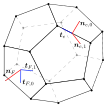
\includegraphics[width=0.3\textwidth]{./figures/hmvem/polygon_normal_vector.pdf}
    \caption{法向和切向的解释.}
    \label{fig:notation}
\end{figure}


给定$d$维多面体$K$,记$\Delta_j(K)$为$K$的所有$j$维面的集合,
其中$j=0,1,\ldots, d-1$。令 $\mathcal{F}^r(K) := \Delta_{d-r}(K)$ 表示 $K$
的所有 $d-r$ 维面的集合,
特别的 $\mathcal{F}(K):=\Delta_{d-1}(K)$
,$\mathcal{E}(K):=\Delta_{d-2}(K)$。对于$\mathcal{F}(K)$中的$F$,
记$\boldsymbol{n}_{K,F}$为指向$\partial
K$的外法向量,若不引起混淆则简记为$\boldsymbol{n}_F$或$\boldsymbol{n}$。
同理 $\bn_{F, e}$ 表示边 $e$ 在 $\partial F$ 上的外法向量,指向 $F$ 的外部。
对于任意 $e \in \mathcal{F}^r(K)$,$e$ 存在 $r$ 个法向和 $d-r$ 个切向,分别记为:
$\{\bn_{F, 1}, \bn_{F, 2}, \ldots, \bn_{F, r}\}$ 和 $\{\bt_{F, 1}, \bt_{F, 2},
\ldots, \bt_{F, d-r}\}$。
特别的对于 $F\in\mathcal{F}^1(K)$,$\boldsymbol{n}_F$ 为其唯一的单位法向量,
对于 $e \in \mathcal{F}^{n-1}(K)$,$\boldsymbol{t}_e$ 为其唯一的单位切向量。
关于法向切向的解释见图 \ref{fig:notation}。

当 $K$ 是一个 $d$ 维的单纯形,记 $F_i\in\mathcal F(K)$ 表示与顶点 $\texttt{v}_i$
对立的 $(d-1)$ 维面,$\boldsymbol n_i$ 表示面 $F_i$ 的单位外法向量,$\lambda_i$
表示与顶点 $\texttt{v}_i$ 对应的点 $\boldsymbol x$ 的重心坐标,其中 $i=0, 1,
\cdots, d$。
显然任取 $d$ 个不同法向 $\{\boldsymbol n_{i_1}, \boldsymbol n_{i_2}, \cdots,
\boldsymbol n_{i_d} \}$ 
都能构成 $\mathbb R^d$ 的基,
$\{\mathrm{skw}({\boldsymbol n_{i_k}\boldsymbol n_{i_l}^{\intercal}})\}_{1\leq
k<l\leq d}$ 构成反对称张量空间 $\mathbb K$ 的基。
对于 $F\in\mathcal F(K)$,令 $\mathcal{E}(F):=\{e\in\mathcal{E}(K): e\subset\partial F\}$。

设 $\{\mathcal {T}_h\}$ 为一族分割 $\Omega$ 为非重叠的简单多面体的分割,其中 $h:=\max\limits_{K\in \mathcal {T}_h}h_K$,
$h_K:=\mbox{diam}(K)$。
使用 $\mathcal F_h^r$ 表示为分割 $\mathcal T_h$ 的所有 $(d-r)$ 维面的集合,其中
$r=1,\ldots,d$。特别地,设 $\mathcal F_h:=\mathcal F_h^1$。
%对于 $\mathcal{T}_h$ 上的分段光滑函数 $v$,定义
%$$
%\|v\|_{\star,h}^2:=\sum_{K\in\mathcal T_h}\|v\|_{\star, K}^2,
%\quad 
%|v|_{\star,h}^2:=\sum_{K\in\mathcal T_h}|v|_{\star,K}^2.
%$$
在面 $F\in\mathcal F_h$ 上,定义 $v$ 的切向梯度和切向散度:
$$
\begin{aligned}
    \nabla_F v&:=\nabla v-(\partial_{\bn} v)\boldsymbol{n} = 
    \sum_{i=1}^{d-1}(\partial_{\bt_{F, i}}v)\boldsymbol{t}_{F, i},\\
\mathrm{div}_F\boldsymbol{v} &
=\mathrm{div}(\boldsymbol{v}-(\boldsymbol{v}\cdot\boldsymbol{n}_{F,
i})\boldsymbol{n}_{F, i})=\mathrm{div}\boldsymbol{v}-\partial_n(\boldsymbol{v}\cdot\boldsymbol{n}).
\end{aligned}
$$

本文中仅考虑星形多面体,下面给出其定义(图 \ref{fig:star}
给出了星形多面体与非星形多面体的例子)。
\begin{definition}[星形多面体]
    对于一个多面体 $K$,如果存在一个点 $\boldsymbol{x}_K$,使得对于任意
    $\boldsymbol{x}\in K$,线段 $\boldsymbol{x}_K\boldsymbol{x}$都在 $K$ 中,
    那么 $K$ 是一个星形多面体。
    所有使 $K$ 星形的点组成的集合的最大内切球半径记为 $\rho_K$,记 $\gamma_K =
    \rho_K/h_K$ 为 $K$ 的 chunkiness 参数。
\end{definition}
\begin{figure}[htbp]
    \centering
\begin{subfigure}[b]{0.4\textwidth}
    \centering
    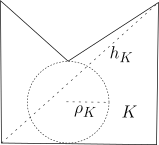
\includegraphics[width=0.6\textwidth]{./figures/star-shaped.pdf}
\end{subfigure}
\begin{subfigure}[b]{0.4\textwidth}
    \centering
    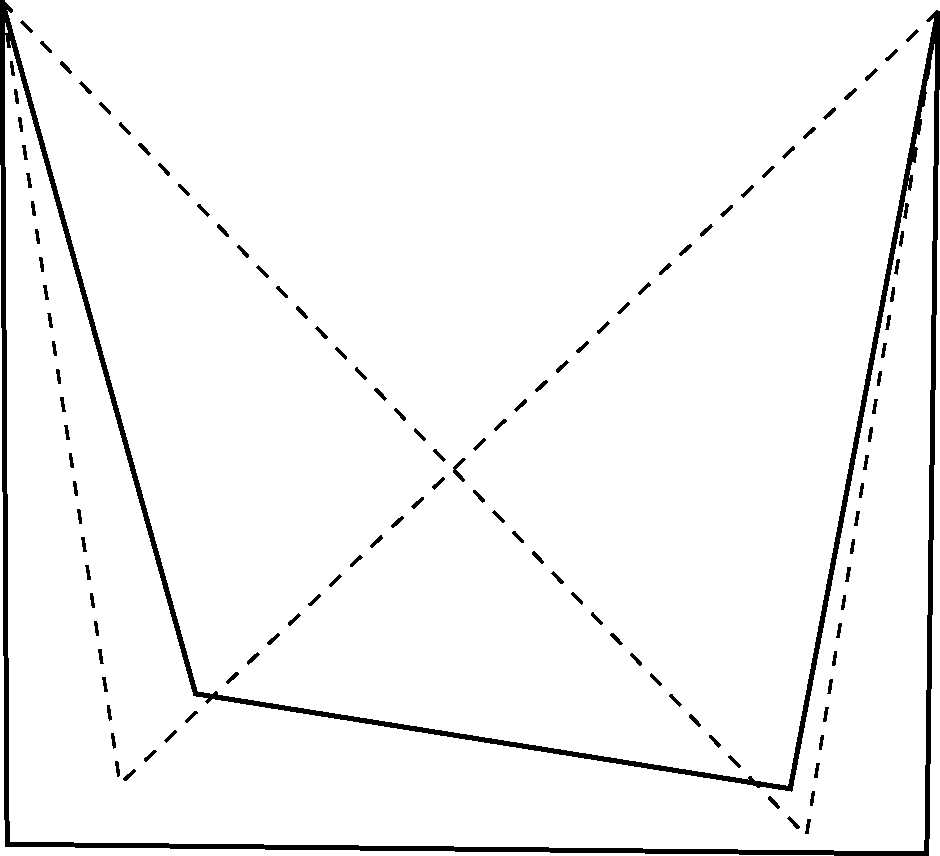
\includegraphics[width=0.6\textwidth]{./figures/no-star-shaped.pdf}
\end{subfigure}
\caption{星形多面体与非星形多面体.}
    \label{fig:star}
\end{figure}



\section{Sobolev 空间}
现在给出本文中使用的一些常用空间的定义和记号。
令 $K$ 是 $\Omega$ 的一个子集,$C_0^{\infty}(K)$ 表示支集属于 $K$ 的无穷光滑函数
组成的线性空间。
$H^m(K)$ 表示 $K$ 上的常规 Sobolev 空间,相应的范数和半范数分别表示为
$\Vert\cdot\Vert_{m,K}$ 和 $|\cdot|_{m,K}$,当 $m$ 为整数时,定义如下:
$$
|v|_{m,K} = \left(\sum_{|\balpha|=m}\int_K
|\partial^{\balpha}v|^2\mathrm{d}x\right)^{1/2}, \quad
\Vert v\Vert_{m,K} = \left(\sum_{|\balpha|\leq m}\int_K
|\partial^{\balpha}v|^2\mathrm{d}x\right)^{1/2}.
$$
当 $m$ 不是整数时,定义如下:
\begin{equation}
\label{fracSobolev}
|v|_{m,K} = \left(\int_K \int_K \frac{ |u(\bfx) - u(\bfy)|^2 }{ |\bfx -
\bfy|^{2(1+m)} } \dd \bfx \dd \bfy\right)^{\frac{1}{2}}, \quad 
\| v \|_{m,K} = \| v \|_{0,K} + |v|_{m,K}.
\end{equation}

当 $K = \Omega$ 时,我们将 $\Vert\cdot\Vert_{m,K}$ 和 $|\cdot|_{m,K}$
简记为 $\Vert\cdot\Vert_{m}$ 和 $|\cdot|_{m}$。 $L^2(K)$ 就是
$H^0(K)$,$(\cdot, \cdot)_K$ 表示 $L^2(K)$ 上的标准内积:
$$
(v, w)_K = \int_K vw\mathrm{d}x.
$$
$\bH^s(K): = H^s(K)\otimes \mathbb{R}^d$为向量Sobolev空间。
$H_0^m(K)$ 表示$H^m$ 空间的迹零子空间,
是$\mathcal C_0^{\infty}(K)$ 相对于范数 $\Vert\cdot\Vert_{m,K}$ 的
闭包。$L_0^2(K)$ 表示 $L^2(K)$ 中所有积分为零的函数组成的空间:
$$
L_0^2(K) = \{v\in L^2(K): \int_K v\mathrm{d}x = 0\}.
$$
$\boldsymbol{H}(\mathrm{div}, K)$ 和 $\boldsymbol{H}_0(\mathrm{div},
K)$ 表示标准的散度向量空间,对应的范数为:
$$
|\boldsymbol{v}|_{\mathrm{div}, K} = \|\diver \bv\|_{0, K}\quad
\Vert\boldsymbol{v}\Vert_{\mathrm{div}, K} = \|v\|_{0,K} +
|\boldsymbol{v}|_{\mathrm{div}, K}.
$$
$\boldsymbol{H}(\bcurl, K)$ 和 $\boldsymbol{H}_0(\bcurl,
K)$ 表示三维的旋度向量空间,对应的范数为:
$$
|\boldsymbol{v}|_{\bcurl, K} = \|\bcurl \bv\|_{0, K}\quad
\Vert\boldsymbol{v}\Vert_{\bcurl, K} = \|v\|_{0,K} +
|\boldsymbol{v}|_{\bcurl, K}.
$$
在二维情况下,
$\bH(\rot;K)$ 表示满足 $\rot$ 值属于 $L^2(K)$ 的 $L^2(K, \mathbb{R}^2)$
的子空间,对应的范数为:
$$
|\bv|_{\rot;K} = \|\rot \bv\|_{0,K}, \quad \|\bv\|_{\rot;K} =
\|\bv\|_{0,K} + |\bv|_{\rot,K}.
$$
进一步的我们定义 $\bH^m(\rot;K)$
$$
\bH^s(\rot;K) = \{ \bu \in \bH^s(K): \rot \bu \in H^s(K) \}.
$$
对应的范数为:
$$
\|\bv\|_{m,\rot;K} = \| \rot \bv \|_{m,K} + \| \bv \|_{m,K}.
$$
定义以下含变系数 $c$ 的空间:
\begin{subequations}
\label{spaces}
\begin{align}
& \bH(\dd^0;\Omega) = \{ \bu \in \bH(\dd;\Omega) : \dd \bu = 0 \} ~~~ \dd = \rot ~ \text{ or } ~ \ddiv,  \label{spaces1} \\
& \bH(c, \dd  ;\Omega) = \{ \bu: c \bu \in \bH(\dd;\Omega)  \} ~~~ \dd = \rot ~ \text{ or } ~ \ddiv \label{spaces2} , \\
& \bH(c, \dd^0  ;\Omega) = \{ \bu: c \bu \in \bH(\dd;\Omega) : \dd (c\bu) = 0
\} ~~~ \dd = \rot ~ \text{ or } ~ \ddiv \label{spaces3}.
\end{align}
\end{subequations}

对于多项式函数,我们定义
$\mathbb P_k(K)$ 为 $K$ 上次数不超过 $k$
的所有多项式组成的线性空间,当 $k < 0$ 时,$\mathbb P_k(K) = \{0\}$。
对于非负整数$k$和$m$,令$\mathbb{P}_{k-2m}^{\perp}(K) \subseteq
\mathbb{P}_k(K)$ 表示 $\mathbb{P}_{k-2m}(K)$在$\mathbb{P}_k(K)$中的
$L^2$
正交补空间。

对于 Banach 空间 $B(K)$,记$B(K; \mathbb{X}):=B(K)\otimes\mathbb{X}$ 表示
函数值在 $\mathbb{X}$ 中的 Banach 空间,
其中$\mathbb{X}$ 为某个张量空间,
如反对称矩阵空间 $\mathbb{K}$、对称矩阵空间 $\mathbb{S}$,
如 $\mathbb{P}_k(K; \mathbb{K})$ 表示 $K$ 上所有分量为不超过 $k$ 次多项式的
反对称矩阵函数组成的线性空间。


\section{常用不等式}
本小节介绍本文中常用的不等式:
\begin{lemma}[Young's 不等式]
    对于任意实数 $a, b > 0$,对于任意的实数 $c>0$,有
    $$
    ab\leq \frac{c}{2}a^2 + \frac{1}{2c}b^2.
    $$
\end{lemma}
\begin{lemma}[Cauchy-Schwarz 不等式]
    令 $A$ 是一个 Hilbert 空间,$(\cdot, \cdot)_A, \|\cdot\|_A$ 分别是
    $A$ 上的内积与范数,那么对于任意 $u, v\in A$,有
    $$
    (u, v)_A \leq \|u\|_A\|v\|_A.
    $$
\end{lemma}
\begin{lemma}[Sololev 空间插值不等式] %TODO
    对于任意 $v \in H^{k+\theta}(K)$,其中 $0\leq \theta\leq 1$,有
    $$
    |v|_{k+\theta, \Omega} \leq |v|_{k, \Omega}^{1-\theta}|v|_{k+1,
    \Omega}^{\theta}.
    $$
\end{lemma}

下面给出 \cite{Grisvard1985} 中关于星形多面体的一些理论。
假设 $K$ 是一个多面体,
令 $\mathfrak{B}_K$ 为 $K$ 的最大内接球,
那么存在 $\mathfrak{B}_K$ 到 $K$ 之间的一个同胚映射
$\boldsymbol{\Phi}_K$,这个映射和其逆映射的 $W^{1, \infty}$ 范数
$|\boldsymbol{\Phi}|_{W^{1,\infty}}$ 和 $|\boldsymbol{\Phi}^{-1}|_{W^{1,
\infty}}$ 是有界的,仅与 $K$ 的 chunkiness 参数 $\gamma_K$ 有关。
根据这个映射可以将 $K$ 上的函数 $v$ 拉回到 $\mathfrak{B}_K$ 得到 $v\circ
\boldsymbol{\Phi}_K$,
关于 $\boldsymbol{\Phi}_K$ 的性质如下:
\begin{property}
$$
\begin{aligned}
    \Vert v \Vert_{0, \partial K} & \eqsim \Vert v\circ \boldsymbol{\Phi}_K
    \Vert_{0, \partial \mathfrak{B}_K} \quad \forall v \in L^2(\partial K),\\
    \Vert v \Vert_{0, K} & \eqsim \Vert v \circ \boldsymbol{\Phi}_K 
    \Vert_{0, \partial \mathfrak{B}_K} \quad \forall v \in L^2(K),\\
    |v|_{1, \partial K} & \eqsim |v\circ \boldsymbol{\Phi}_K|_{1, \partial \mathfrak{B}_K} \quad 
    \forall v \in H^1(\partial K), \\
    |v|_{1, K} & \eqsim |v\circ \boldsymbol{\Phi}_K|_{1, \mathfrak{B}_K} \quad 
    \forall v \in H^1(K), \\
    |v|_{1/2, \partial K} & \eqsim |v\circ \boldsymbol{\Phi}_K|_{1/2, \partial \mathfrak{B}_K} \quad 
    \forall v \in H^{1/2}(\partial K). \\
\end{aligned}
$$
等价性中的参数仅与 $\gamma_K$ 有关,与 $h_K$ 无关。
\end{property}
下面给出一些关于 $d$ 维星形多面体 $K$ 上 Sobolev 空间的不等式,
这些不等式中的常数 $C$ 同样仅依赖于 chunkiness 参数 $\gamma_K$。注意
Poincar\'e-Friedrichs 不等式中的参数与 $\gamma_K$ 无关。
\begin{lemma}[Poincar\'e-Friedrichs 不等式]
    对于任意 $u\in H^1_0(K)$ 有\cite{2003Henrot}:
    \begin{equation}
    \label{eq:Poincare-Friedrichs2}
    \|u\|_{0, K} \leq (\sqrt{\pi}j_0)^{-1}|K|^{\frac{1}{2}}|u|_{1, K}.
    \end{equation}
    其中的常数为中 Dirichlet-Laplacian 算子的第一特征值的倒数,
    $j_0\approx 2.4$ 是第一类 Bessel 函数 $J_0$ 的第一个零点。
    对于 $u\in H^1(K)$ 有\cite[定理 3.2]{2005ZhegQi}:
    \begin{equation}
        \label{eq:Poincare-Friedrichs1}
        \|u\|_{0, K} \leq 2h_K^{1+\frac{d}{2}}|K|^{-\frac{1}{2}}|u|_{1, K} + 
        |K|^{\frac{1}{2}}\left|\int_{K}u\mathrm{d}x\right|.
    \end{equation}
\end{lemma}
\begin{lemma}[多项式逆不等式]
    \cite[引理10]{Huang2020}\cite[引理2.1]{2021WeiHuangLi}
    对于任意非负整数 $j, k$,任意多项式 $v\in \mathbb P_k(K)$ 满足
    \begin{equation}
    \label{eq:polyinverse}
    \begin{aligned}
    \Vert v\Vert_{0, K} \leq Ch^{-j}_K|v|_{-j, K}
    \end{aligned}
    \end{equation}
\end{lemma}
\begin{lemma}[迹不等式]
    对于任意 $v\in H^1(K)$,存在一个常数 $C$ 仅依赖于 $K$ 和 $m$,使得
    \begin{equation}
        \label{L2trace}
    \|v\|_{0, \partial K}^2 \leq C h_K^{-1}\|v\|_{0, K} + Ch_K|v|_{1, K}.
    \end{equation}
\end{lemma}
\begin{lemma}[乘型迹不等式]\cite[Theorem 1.5.1.10]{Grisvard1985}
    \label{lemma:multiplicative_trace}
    对于任意 $v\in H^1(K)$ 有:
    \begin{equation}
    \label{eq:multiplicative_trace}
    \begin{aligned}
    \|v\|_{0, \partial K}^2 \leq Ch_K^{-1}\|v\|_{0, K}(h_K|v|_{1, K} + \|v\|_{0, K}).
    \end{aligned}
    \end{equation}
\end{lemma}
\begin{lemma}[逆迹定理]
    存在一个 $H^{1/2}(\partial K)$ 到 $H^1(K)$ 的线性算子 $\tr^{*}$ 使得:
    \begin{itemize}
        \item $\tr(\tr^{*} v) = v \quad \forall v \in H^{1/2}(\partial K)$.
        \item $h^{-1}_K \| \tr^* v \|_{0, K} + |\tr^* v|_{1, K} \leq
            C |v|_{1/2. \partial D}$.
    \end{itemize}
\end{lemma}
\begin{lemma}[$L^2$ 投影估计]
    令 $Q_k^K$ 是 $L^2(K)$ 到 $\mathbb P_k(K)$ 的 $L^2$ 投影,那么 
    对于任意 $v\in H^j(K)$,$0\leq i\leq j\leq k+1$,有
    \begin{equation}
        \label{eq:l2projectionestimate}
    h_K^i|v - Q_k^K v|_{i, K} + h_K^{1/2}|v - Q_k^K v|_{0, \partial K}
    \leq Ch_K^{j}|v|_{j, K}.
    \end{equation}
\end{lemma}


%\section{Sobolev 空间}
%\begin{definition}[弱导数]
%    令 $\Omega$ 是一个 $\mathbb R^n$ 中的开集, $\alpha$ 是一个多重指标,
%    $u \in L_{loc}^1(\Omega)$, 若存在 $v\in L_{loc}^1(\Omega)$ 
%    使得对于任意 $\phi \in C_0^{\infty}(\Omega)$ 满足:
%    $$
%    \int_{\Omega} u D^{\alpha}\phi \mathrm{d}x = (-1)^{|\alpha|}\int_{\Omega}
%    v\phi \mathrm{d}x 
%    $$
%    则称 $v$ 是 $u$ 的 $\alpha$ 阶弱导数,记作 $D^{\alpha}u$.
%\end{definition}
%
%\begin{definition}[整数 Sobolev 空间]
%    令 $\Omega$ 是一个 $\mathbb R^n$ 中的开集,$k$ 是一个非负整数,定义
%    $$
%    H^k(\Omega) = \{u \in L^2(\Omega): D^{\alpha}u \in L^2(\Omega), |\alpha| \leq k\}
%    $$
%    其中 $|\alpha| = \alpha_0 + \alpha_1 + \cdots + \alpha_{n-1}$.
%\end{definition}
%
%\begin{definition}[分数 Sobolev 空间]
%    令 $\Omega$ 是一个 $\mathbb R^n$ 中的开集,$s$ 是一个实数,定义
%    $$
%    H^s(\Omega) = \{u \in L^2(\Omega): \int_{\Omega}\int_{\Omega}
%    \frac{|u(x) - u(y)|^2}{|x-y|^{n+2s}} \mathrm{d}x\mathrm{d}y < \infty\}
%    $$
%\end{definition}

%\begin{definition}[半整数 Sobolev 空间]
%    令 $\Omega$ 是一个 $\mathbb R^n$ 中的开集,$s$ 是一个实数,定义
%    $$
%    H^s(\Omega) = \{u \in L^2(\Omega): \int_{\Omega}\int_{\Omega}
%    \frac{|u(x) - u(y)|^2}{|x-y|^{n+2s}} \mathrm{d}x\mathrm{d}y < \infty\}
%    $$
%\end{definition}
%
%\begin{theorem}[迹不等式]
%\end{theorem}
%
%\begin{theorem}[Poincar\'e 不等式]
%    令 $\Omega$ 是一个有界开集,$u \in H_0^1(\Omega)$, 则
%    $$
%    \int_{\Omega} |u|^2 \mathrm{d}x \leq C \int_{\Omega} |\nabla u|^2 \mathrm{d}x
%    $$
%\end{theorem}
%
%
%\begin{theorem}[多项式逆不等式]
%    令 $K$ 是一个多面体,
%\end{theorem}


